% !Mode:: "TeX:UTF-8"
% 七年级上学期第一单元三视图

\begin{defproblem}{7NJ-01-01}%
\begin{onlyproblem}%
在利用三视图确定小木块个数时,数字一般标在\underline{\hspace*{2cm}}图上.

\end{onlyproblem}%
\begin{onlysolution}%
\begin{solution}%%
俯视
\end{solution}%
\end{onlysolution}%
\end{defproblem}





\begin{defproblem}{7NJ-01-02}%
\begin{onlyproblem}%
观察一个几何体的形状通常从三个方向看,从正面看(主视图),从左面看(左视图),从上面看(俯视图),

从正面看可以看到几何体的\underline{\hspace*{2cm}}和\underline{\hspace*{2cm}};

从左面看可以看到几何体的\underline{\hspace*{2cm}}和\underline{\hspace*{2cm}};

从上面看可以看到几何体的\underline{\hspace*{2cm}}和\underline{\hspace*{2cm}}.
\end{onlyproblem}%
\begin{onlysolution}%
\begin{solution}%%
从正面看可以看到几何体的列数和层数;
从左面看可以看到几何体的行数和层数;
从上面看可以看到几何体的列数和行数.
\end{solution}%
\end{onlysolution}%
\end{defproblem}




\begin{defproblem}{7NJ-01-03}%
\begin{onlyproblem}%
如图是一个由多个相同小立方块堆积而成的几何体的俯视图,图中所示数字为该位置小立方块的个数,则这个几何体的主视图是(    )
\begin{center}
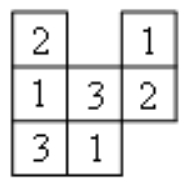
\includegraphics[width=2cm]{7NJ01-01-20190802-1.jpg}
\end{center}

\begin{center}
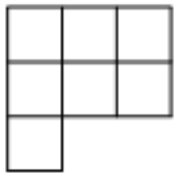
\includegraphics[width=2cm]{7NJ01-01-20190802-2.jpg}
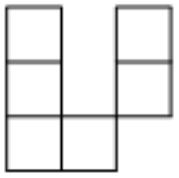
\includegraphics[width=2cm]{7NJ01-01-20190802-3.jpg}
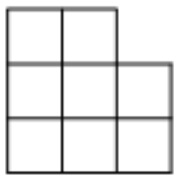
\includegraphics[width=2cm]{7NJ01-01-20190802-4.jpg}
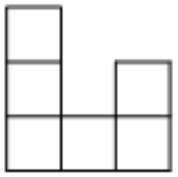
\includegraphics[width=2cm]{7NJ01-01-20190802-5.jpg}
\end{center}

\end{onlyproblem}%
\begin{onlysolution}%
\begin{solution}%%
C
\end{solution}%
\end{onlysolution}%
\end{defproblem}




\begin{defproblem}{7NJ-01-04}%
\begin{onlyproblem}%
如图所示是由一些相同的小正方体构成的几何体的三视图,则这些相同的小正方体的个数是(    )
\begin{center}
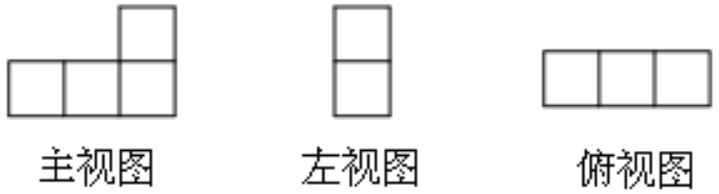
\includegraphics[width=5cm]{7NJ01-01-20190802-6.jpg}
\end{center}

\xx
{3个}
{4个}
{5个}
{6个}

\end{onlyproblem}%
\begin{onlysolution}%
\begin{solution}%%
B
\end{solution}%
\end{onlysolution}%
\end{defproblem}



\begin{defproblem}{7NJ-01-05}%
\begin{onlyproblem}%
如图所示是由一些相同的小正方体构成的几何体的三视图,这些相同的小正方体的个数是(    )
\begin{center}
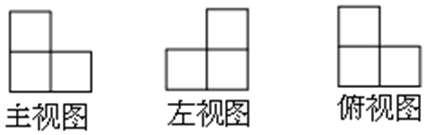
\includegraphics[width=5cm]{7NJ01-01-20190802-7.jpg}
\end{center}

\xx
{3个}
{4个}
{5个}
{6个}

\end{onlyproblem}%
\begin{onlysolution}%
\begin{solution}%%
B
\end{solution}%
\end{onlysolution}%
\end{defproblem}




\begin{defproblem}{7NJ-01-06}%
\begin{onlyproblem}%
用小正方体搭建成的几何体,下面三个图分别是它的主视图、左视图和俯视图,那么构成这个几何体的小正方体有(    )
\begin{center}
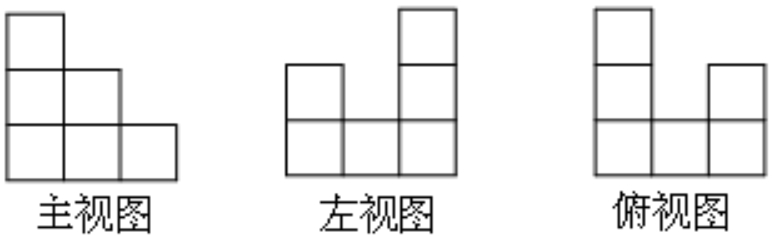
\includegraphics[width=5cm]{7NJ01-01-20190802-8.jpg}
\end{center}

\xx
{6个}
{9个}
{10个}
{11个}

\end{onlyproblem}%
\begin{onlysolution}%
\begin{solution}%%
B
\end{solution}%
\end{onlysolution}%
\end{defproblem}



\begin{defproblem}{7NJ-01-07}%
\begin{onlyproblem}%
由若干个相同的小正方体搭成的一个几何体的主视图和俯视图如图所示,则组成这个几何体的小正方体的个数最少有(    )
\begin{center}
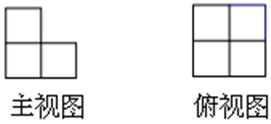
\includegraphics[width=5cm]{7NJ01-01-20190802-9.jpg}
\end{center}

\xx
{4个}
{5个}
{6个}
{7个}


\end{onlyproblem}%
\begin{onlysolution}%
\begin{solution}%%
B
\end{solution}%
\end{onlysolution}%
\end{defproblem}




\begin{defproblem}{7NJ-01-08}%
\begin{onlyproblem}%
如图是由一些大小相同的小正方体搭成的一个几何体的左视图和俯视图,则组成这个几何体的小正方体的个数最多有(    )
\begin{center}
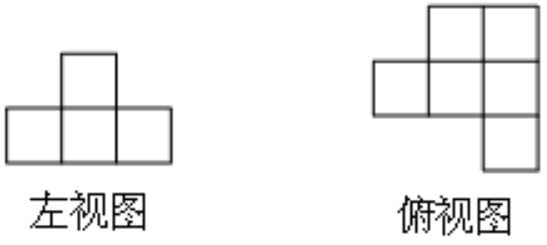
\includegraphics[width=5cm]{7NJ01-01-20190802-10.jpg}
\end{center}

\xx
{5个}
{6个}
{8个}
{9个}


\end{onlyproblem}%
\begin{onlysolution}%
\begin{solution}%%
C
\end{solution}%
\end{onlysolution}%
\end{defproblem}



\begin{defproblem}{7NJ-01-09}%
\begin{onlyproblem}%
用小正方体积木搭出一个主视图和俯视图如图所示的几何体,它最多需要(    )个小正方体积木.
\begin{center}
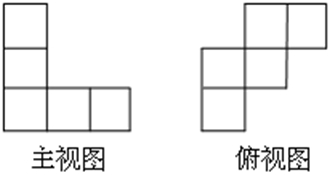
\includegraphics[width=5cm]{7NJ01-01-20190802-11.jpg}
\end{center}

\xx
{8个}
{9个}
{10个}
{11个}


\end{onlyproblem}%
\begin{onlysolution}%
\begin{solution}%%
B
\end{solution}%
\end{onlysolution}%
\end{defproblem}






